\chapter{Výpočetní část}

\section{Tvorba geometrie a výpočetní sítě}

Prvním krokem před každou CFD simulací je tvorba geometrie systému a její následná diskretizace (tzv. vysíťování). Výpočetní doména byla vytvořena podle geometrie experimentu uvedené v~kapitole \ref{chap:exp} prostřednictvím programu ANSYS DesignModeler 12.1. Pro snížení výpočetní náročnosti byla simulována pouze část nádrže obsahující kapalinu bez přítomnosti vzduchu. Míchací nádoba byla rozdělena na část rotační, kterou tvořil válec o~výšce \SI{5.2}{\centi\meter} a průměru \SI{16.5}{\centi\meter}. Zmíněná rotační doména obsahující míchadlo a část hřídele začínala ve vzdálenosti \SI{1.35}{\centi\meter} od spodní hrany míchadla. Zbývající část systému obsahující větší část hřídele, dno, stěny a narážky nádoby představovala stacionární oblast. Vytvořená geometrie systému je znázorněna na obr. \ref{fig:geo}, kde zelenou barvou je znázorněna rotační zóna kolem míchadla. 

\begin{figure}[h!]
\centering
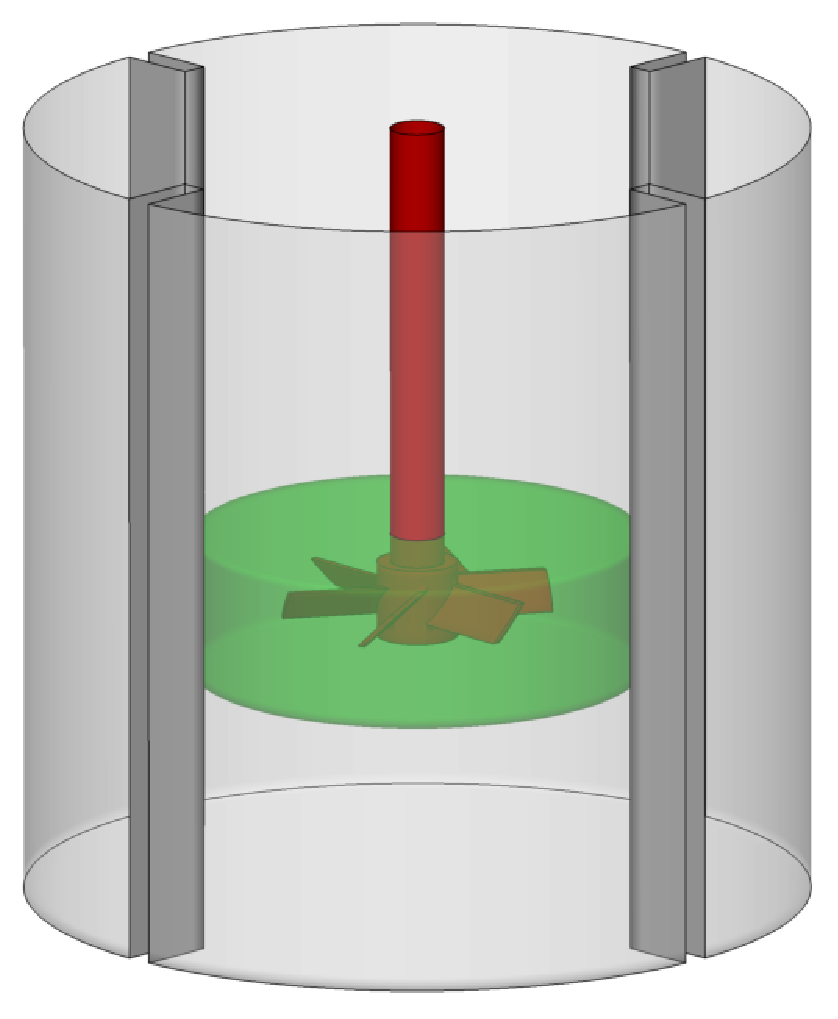
\includegraphics[scale=0.5]{images/geo.eps}
\caption{Geometrie systému}
\label{fig:geo}
\end{figure} 

Pro tvorbu výpočetní sítě byl využit program ANSYS Meshing 12.1 do kterého byla načtena geometrie nádoby vytvořená v~předcházejícím kroku. Výsledná nestrukturovanou síť se skládala z \num{264398} buněk o~průměrném objemu \SI{0.07}{\milli\litre}. Jednalo se převážně o~šestistěnné buňky, přičemž pouze v~oblasti pod míchadlem se vyskytovalo \num{132} třístěnných hranolů. Řez diskretizovanou doménou je zachycen na obr. \ref{fig:mesh} ze kterého si lze povšimnout, že ve spodní části nádoby je síť úmyslně zahuštěna. 
\begin{figure}[t]
\centering
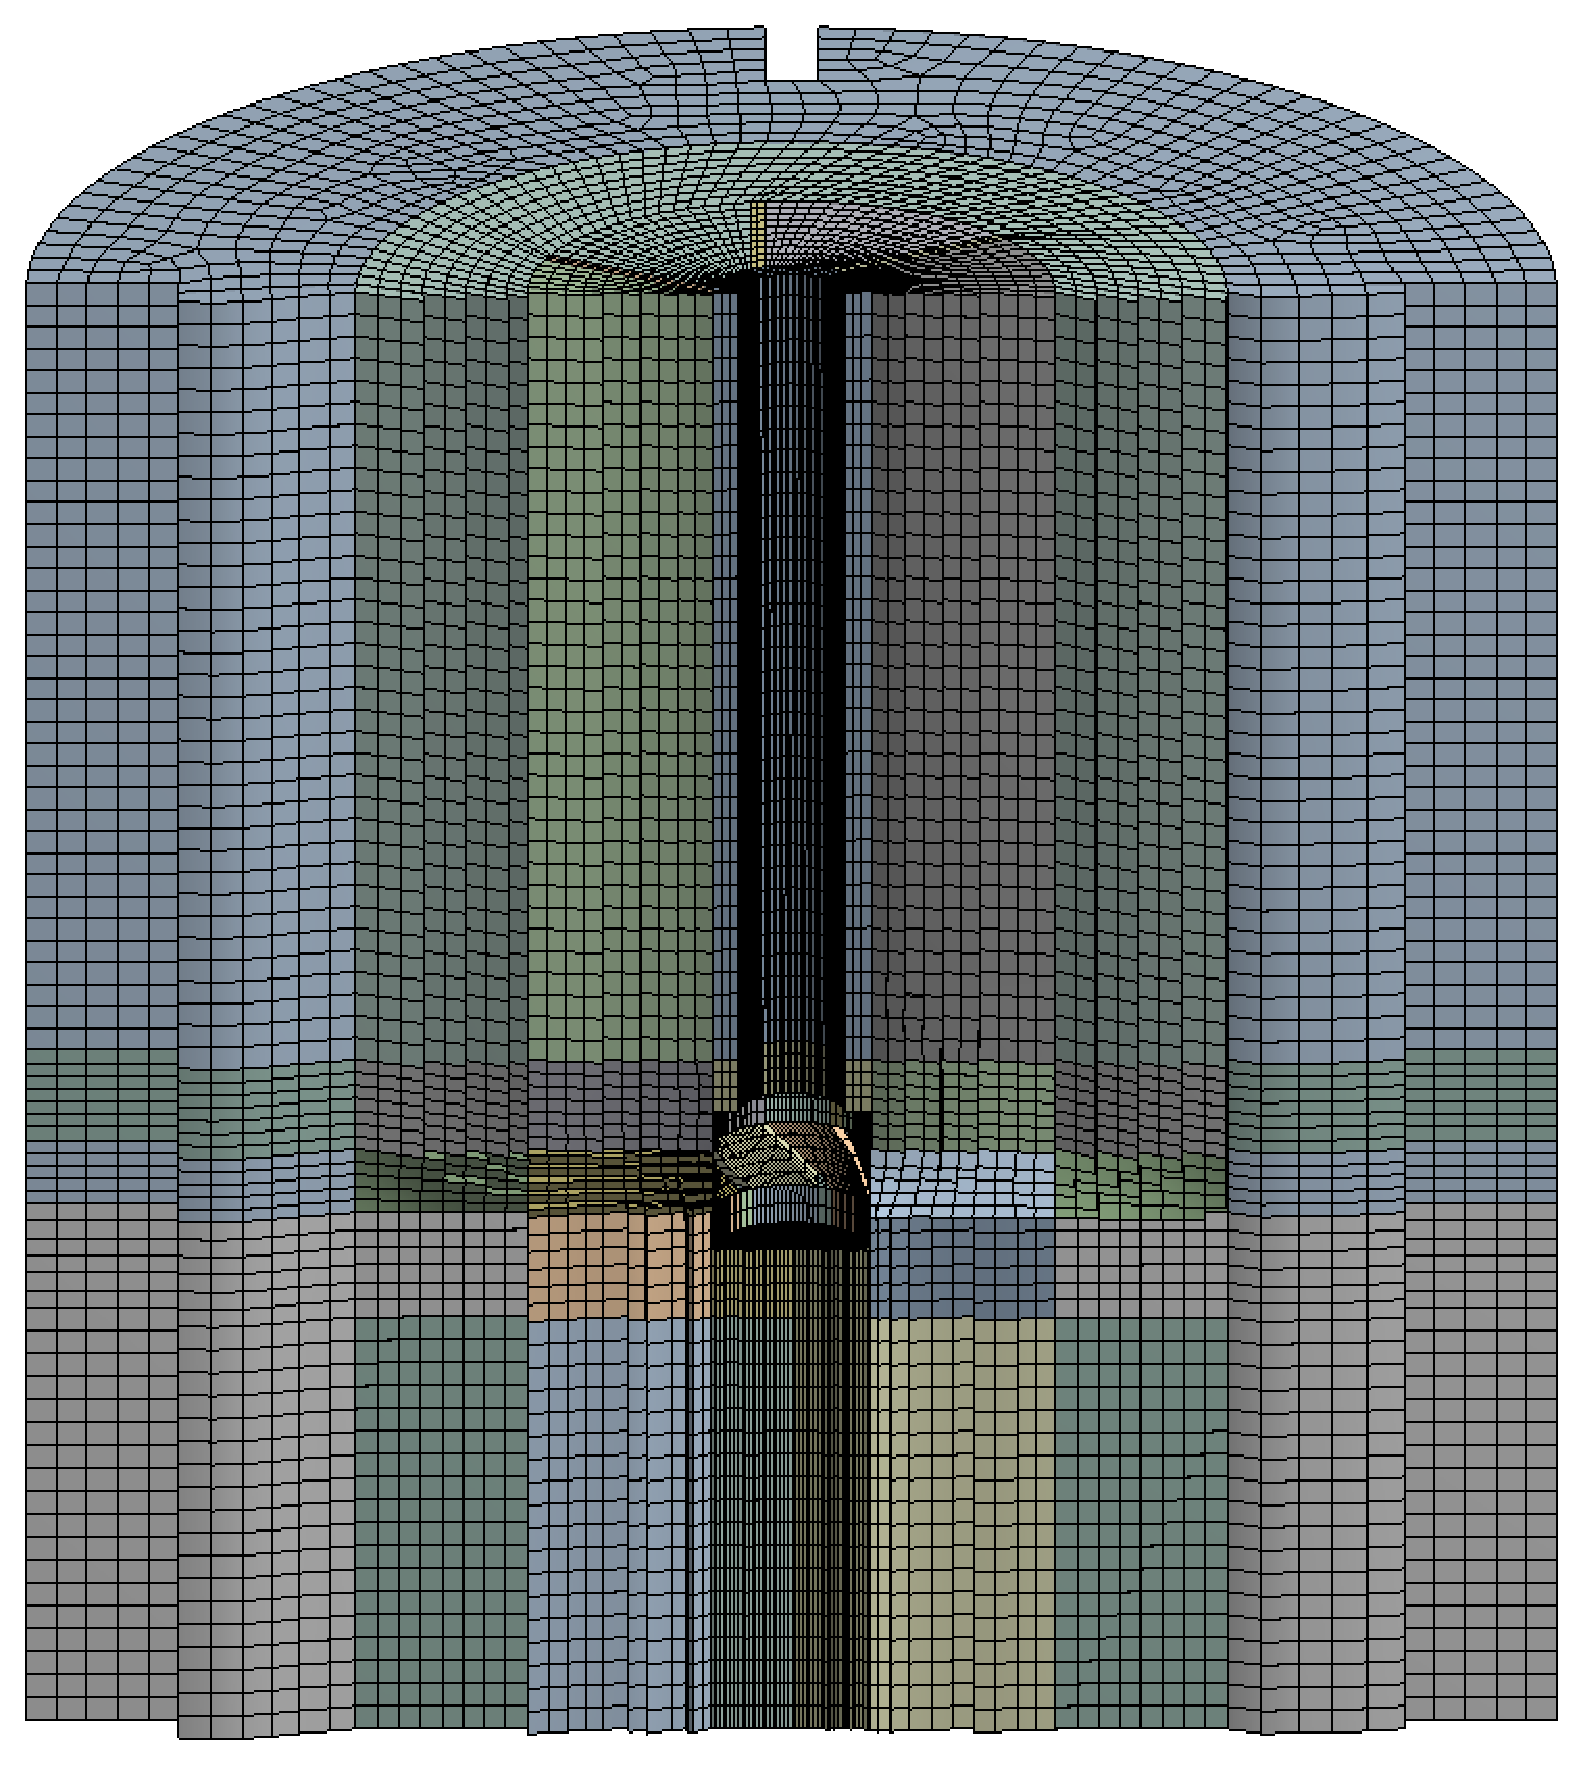
\includegraphics[scale=0.28]{images/mesh.eps}
\caption{Řez výpočetní sítí}
\label{fig:mesh}
\end{figure} 
Pro posouzení kvality vytvořené sítě existuje celá řada kritérií, avšak mezi jedno z nejpoužívanější patří tzv. šikmost (angl. skewness) definovaná jako:
\begin{equation}
      skewness = \mathsf{max}\kula{\frac{\beta_{max} - \beta_{e}}{180 - \beta_{e}}, \frac{\beta_{e} - \beta_{min}}{\beta_{e}}}
  	\label{eq:skw}
\end{equation} 
kde $\beta_{min}$, $\beta_{max}$ značí nejmenší resp. největší úhel v~buňce a $\beta_{e}$ představuje úhel v~pravidelném (ideálním) elementu. Šikmost se obecně pohybuje v~intervalu od \num{0} do \num{1}, přičemž nulová hodnota značí nejlepší kvalitu buňky, a naopak šikmost rovna jedné indikuje úplnou degeneraci elementu. Vybrané charakteristiky této veličiny pro vytvořenou výpočetní doménu jsou uvedeny v~tabulce \ref{tab:skw_tab}. Z~uvedených hodnoty vyplývá, že vygenerovaná síť dosahuje výborné kvality.
\begin{table}[h!]
\centering
\caption{Charakteristiky šikmosti pro vytvořenou síť}
\label{tab:skw_tab}
\begin{tabular}{lr}
\toprule
\textbf{Charakteristika} & \textbf{Hodnota} \\
\midrule

Maximální šikmost & \num{0.666} \\
Průměrná šikmost & \num{0.164} \\
Směrodatná odchylka šikmosti & \num{0.123} \\

\bottomrule
\end{tabular}
\end{table}

\section{Uživatelem definované funkce}
Uživatelem definované funkce (UDF) jsou moduly načítané do softwaru \flu, jenž rozšiřují nebo upravují schopnosti řešiče. Například může se jednat o~vytvoření vlastních počátečních a okrajových podmínek, změnu materiálových vlastností a modifikaci simulačních modelů. Pro tvorbu zdrojových souborů se využívá programovací jazyk C. Vytvořené soubory jsou následně zkompilovaný do dynamické knihovny.

Právě pomocí uživatelem definovaných funkcí byly implementovány modely pro koeficient odporu uvedené v~tabulce \ref{tab:cds} spolu s~klasickým modelem dle Schillera a Neumanna (\ref{eq:schlneu}). Navíc kromě korelací pro výpočet součinitele odporu byla do této knihovny naprogramována funkce pro výpočet kvality suspenze podle vztahu \ref{eq:kvasus}. Všechny vytvořené zdrojové kódy jsou uvedeny v~kapitole \nameref{sec:priloha}.

\section{Vlastní CFD simulace}
Ke studiu suspendace pomocí CFD simulaci byl využit komerční software \flu{} 12.1.4 do kterého byla načtena vytvořená výpočetní síť. Následně byly nastaveny okrajové podmínky pro jednotlivé části řešené domény. Pro všechny fyzické části nádrže (dno, stěny, narážky, hřídel a míchadlo) byla vybrána okrajová podmínka typu stěna pro kterou platí, že rychlost proudění na jejím povrchu je nulová. Z~důvodu jednoduchosti byla pro hladinu kapaliny zvolena okrajová podmínka symetrie, jenž vyjadřuje nulovou hodnotu gradientu pro jednotlivé veličiny. Tato volba je obvyklá pro systémy kde je pozornost věnována dějům probíhající uvnitř nádoby, a nikoliv na mezifázovém rozhraní, což je právě případ suspendace. Pohyb rotační části domény byl v~případě stacionární simulace modelován pomocí metody vícenásobných souřadnicových soustav (MRF) a pro nestacionární (dynamickou) simulaci byla použita technika klouzající sítě (SM). 

Proudění v~nádobě bylo považováno za izotermní, nestlačitelné a plně turbulentní. Pro popis turbulence byl využit standardní \keps{} turbulentní model s~disperzní modifikací pro vícefázový systém. Navíc během simulace byl zohledněn efekt turbulentní disperze dle doporučení autorů \citet{lju01} nebo \citet{tamb09}. Z~mezifázových sil byla modelována pouze odporová síla jakožto dominantní člen. Pro popis koeficientu odporu byly využity korelace dodané v~podobě UDF knihovny. V~provedených simulacích byla největší pozornost věnována modelu dle Khopkara, který byl navržen speciálně pro CFD simulaci suspendace v~míchaných nádobách.

Pro popis vícefázového proudění v~nádrží byl použit 
matematický model Eulerian-Eulerian, přičemž jako primární fáze 
byla volena voda nebo PVP a sekundární fázi tvořily kuličky z~PVC. 
Při použití této techniky se pevná fáze modeluje jako ideální 
kapalina (bez vnitřního tření). Zmíněnou skutečnost bylo třeba 
zohlednit během nastavení simulace. Viskozita pevné fáze byla proto zvolena téměř nulová ($\SI{e-10}{\pascal\second}$) a jednotlivé složky tečného napětí na všech stěnách byly rovněž nastaveny na nulu. Pro porovnání byly rovněž některé výpočty provedeny s~vícefázovým přístupem Eulerian-Granular. Hodnota viskozity zrnité fáze byla určena pomocí vztahů navržených \citet{syam93}. Členy jako radiální distribuční funkce, tlak pevné fáze a dilatační viskozita byly stanoveny pomocí modelů, jenž navrhli autoři \citet{lun84}.  

Vlastní CFD výpočet byl proveden jako nestacionární, aby bylo možné sledovat průběh suspendace a dynamiku vzniku suspenzního mraku. Na začátku každé simulace byla na dno nádoby umístěná pevná fáze o~zvolené koncentraci 5, 10 nebo \volproc{15}. Pro potřeby počáteční podmínky bylo zvolené nulové rychlostní pole spolu s~hodnotou turbulentní kinetické energie rovnu \SI{e-3}{\meter\squared\per\second\squared} a její rychlosti disipace \SI{e-3}{\meter\squared\per\second\cubed}. K~určení rychlostního a tlakového pole byla využita vícefázová modifikace algoritmu SIMPLE. Velikost časového kroku byla zvolena \SI{0.001}{\second}, přičemž v~každém kroku bylo provedeno maximálně \num{55} iterací. Konvergenční kritérium bylo splněno pokud hodnoty reziduí všech řešených veličin byly menší než \num{e-3}. Pro sledování konvergence výpočtu byla také monitorována síla působící na narážky nádoby a průměrná hodnota koeficientu odporu v celém systému. V~prvních \num{100} časových krocích byly použity diskretizační náhrady pouze prvního řádu a podrelaxační faktory pro tlak, hybnost a turbulentní viskozitu byly sníženy na hodnotu \num{0.2}, \num{0.2} respektive \num{0.8}. Po této době následovalo přepnutí na diskretizační náhrady druhého řádu a nastavení všech podrelaxčních faktorů na své výchozí hodnoty. Celková doba simulace činila \SI{7}{\second}, což se dle experimentů jevila jako dostatečná doba k~ustálení tokového pole. Simulace probíhala na počítači HP Z600 osazený dvěma procesory Intel Xeon X5570 a pamětí 24~GB s~operačním systémem CentOS 5.3 x86-64. Doba výpočtu jedné reálné vteřiny trvala přibližně 4 hodiny.

Získaná rychlostí pole byla poté využita ke stanovení doby homogenizace. Stopovací látka s fyzikálními vlastnostmi stejnými jako kapalná fáze byla na počátku simulace umístěna \SI{2}{\centi\meter} po hladinu vsádky. V průběhu výpočtu byly následně zaznamenávány hodnoty objemového zlomku indikační látky v místě umístění vodivostní sondy.


